
\documentclass[12pt]{article}
\usepackage{amsmath}
\DeclareMathOperator*{\argmin}{arg\,min} % thin space, limits underneath in displays
\DeclareMathOperator*{\argmax}{arg\,max} % thin space, limits underneath in displays
\newtheorem{thm}{Theorem}
\usepackage{amssymb}
\usepackage{amsfonts}
\usepackage{mathrsfs}
\usepackage{bm}
\usepackage{indentfirst}
\setlength{\parindent}{0em}
\usepackage[margin=1in]{geometry}
\usepackage{graphicx}
\usepackage{setspace}
\doublespacing
\usepackage[flushleft]{threeparttable}
\usepackage{booktabs,caption}
\usepackage{float}
\usepackage{graphicx}
\usepackage[sort,comma]{natbib}
\usepackage[hidelinks]{hyperref}

\usepackage{import}
\usepackage{xifthen}
\usepackage{pdfpages}
\usepackage{transparent}

\newcommand{\incfig}[1]{%
\def\svgwidth{\columnwidth}
\import{./figures/}{#1.pdf_tex}
}




\title{}
\author{}
\date{}


\begin{document}


\section{CDF and PDF}
CDF:
\begin{equation*}
F_{X}(x) = \int_{ - \infty }^{x}f_{x}(u)du, \quad f_{x}(x) \ge 0, \forall x \in \mathbb{R} 
\end{equation*}


\subsection{Probability model}
Probability model $ \Phi $ is a collection of pdf indexed by a set of unknown parameters
$ \bm{\theta} $; one density for each possible value of $ \bm{\theta} $ in the parameter
space $ \Theta $.
\begin{equation*}
\Phi = \left\{ f(x,\bm{\theta}), \bm{\theta}\in \Theta, x \in \mathbb{R}_{X} \right\} 
\end{equation*}

{\textbf {Support}} of the density $ f_{x}(x) $ is the range of values of the RVs for which the
density function is {\textbf {positive}}.
\begin{equation*}
\mathbb{R}_{X}:=\left\{ x \in \mathbb{R}_{X}: f_{x}(x) > 0 \right\} 
\end{equation*}

Example:

Binomial distribution
\begin{equation*}
\Phi = \left\{ f(x;\theta) = \binom{x}{n}\theta^{x}(1 - \theta)^{n - x},
\theta \in (0,1), x \in [0,n], n = 1,2,...\right\} 
\end{equation*}


\section{Moments}
\begin{equation*}
	E[h(X)] = \int_{ - \infty }^{\infty }h(x)f(x;\bm{\theta})dx, 
\end{equation*}
where $ h(X) $ can be $ X^{r}, e^{tx}, e^{itx} $


\subsection{Mean}
$ h(X):= X , \quad x \in \mathbb{R}_{X}$, 
\begin{align*}
	E(X) &= \int_{ - \infty }^{\infty } x \cdot f_{x}(x;\bm{\theta})dx, \text{ for continuous RVs }\\
	&= \sum\limits_{x_{i}\in \mathbb{R}_{X}} x_{i}\cdot f_{x}(x_{i};\bm{\theta}), \text{ for 
	discrete RVs}
\end{align*}

Properties:
\begin{align*}
E(c)&= c\\
E(aX_1 + bX_2)&= aE(X_1) + bE(X_2)
\end{align*}


\begin{figure}[H]
\center{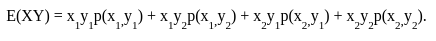
\includegraphics[scale = ]  {figures/E_XY.png}}
\end{figure}




\subsection{Variance}
For calculating the variance, $ h(X):= [X - E(X)]^{2} $
\begin{align*}
	Var(X):=E[(X - E(X))^{2}] &= \int_{ - \infty }^{\infty }(x - \mu)^{2}f_{x}(x;\bm{\theta})dx \\
	&= E(X^{2}) - (E(X))^{2}
\end{align*}

Variance measures the dispersion around the mean.

For {\textbf {independent RVs,}}
\begin{align*}
Var(c) &= 0\\
Var(aX_1 + bX_2)&= a^{2}Var(X_1) + b^{2}Var(X_2), \text{ if $ X_1, X_2 $ are independent }\\
Var \left( \sum\limits_{i = 1} ^n a_{i}X_{i}	 \right) &= \sum\limits_{i = 1} ^n a_{i}^{2}Var(X_{i})	\\
Var(aX + bY) &= a^{2}Var(X) + b^{2}Var(Y) + 2abCov(X,Y), \text{ if X,Y are not independent. }
\end{align*}


{\textbf {Covariance:}}

\begin{align*}
		Cov(X,Y) &= E \left\{ \left[ X - E(X) \right] \left[ Y - E(Y) \right]   \right\} \\
		&= E(XY) - E(X)E(Y)
\end{align*}
{\textbf {Properties:}}
\begin{align*}
		Cov(a,X) &= 0\\
		Cov(X,Y) &= Cov(Y,X)\\
		Cov(aX, bY) &= abCov(X,Y)\\
		Cov(aX + bY, Z) &= aCov(X, Z) + bCov(Y,Z)\\
		Cov(X,Y) &= 0, \text{ if X,Y are independent }
\end{align*}


\noindent\fbox{%
\parbox{\textwidth}{%
\begin{align*}
Cov(aX,bY)&= E \left\{ \left[ aX - E(aX) \right]\left[ bY - E(bY) \right]   \right\} \\
&= E \left\{ aXbY - aXE(bY) - bYE(aX) + E(aX)E(bY) \right\} \\
&= abE(XY) - abE(X)E(Y)\\
&= ab \left[ E(XY) - E(X)E(Y) \right] \\
&= abCov(X,Y)
\end{align*}
\begin{align*}
Cov(X + Y, Z)&= E[(X + Y)Z] - E(X + Y)E(Z)\\
&= E(XZ + YZ) - E(X)E(Z) - E(Y)E(Z)\\
&= E(XZ) - E(X)E(Z) + E(YZ) - E(Y)E(Z)\\
&= Cov(X,Z) + Cov(Y,Z)
\end{align*}
}%
}\\


{\textbf {Note:}} You CANNOT directly compare two covariance because Cov is affected
by the unit of a RV. We need to convert Cov to correlation coefficient.


{\textbf {Population vs Sample Variance Covariance:}}

Population:
\begin{itemize}
\item Mean:
		$ E(X) = \frac{1}{n}\sum\limits_{i = 1} ^n X_{i}	 $, 
		$\quad E(Y) = \frac{1}{n}\sum\limits_{i = 1} ^n Y_{i}	 $
\item Var:
		\begin{equation*}
		Var(X) =\sigma_{X}^{2} =  \frac{\sum\limits_{i = 1} ^n (X_{i} - E(X))^{2}	}{n}, \quad
    Var(Y) =\sigma_{Y}^{2} =  \frac{\sum\limits_{i = 1} ^n (Y_{i} - E(Y))^{2}	}{n}
		\end{equation*}
\item Cov:
		\begin{equation*}
				Cov(X,Y) = \frac{E \left\{ [X - E(X)][Y - E(Y)] \right\} }{n}
				= \frac{\sum\limits_{i = 1} ^n [X_{i} - E(X)][Y_{i} - E(Y)]	}{n}
		\end{equation*}
\item Correlation Coefficient:
		\begin{equation*}
		\rho_{XY} = \frac{Cov(X,Y)}{\sigma_{X}\sigma_{Y}}
		\end{equation*}
\end{itemize}



Sample:
\begin{itemize}
\item Mean:
\begin{equation*}
 \overline{X} = \frac{1}{n}\sum\limits_{i = 1} ^n X_{i}, \quad	
\overline{Y} = \frac{1}{n}\sum\limits_{i = 1} ^n Y_{i}
\end{equation*}

\item Var:
		\begin{equation*}
		Var(X) =s_{X}^{2} =  \frac{\sum\limits_{i = 1} ^n (X_{i} -  \overline{X})^{2}	}{n - 1}, \quad
    Var(Y) =s_{Y}^{2} =  \frac{\sum\limits_{i = 1} ^n (Y_{i} -  \overline{Y})^{2}	}{n - 1}
		\end{equation*}
\item Cov:
		\begin{equation*}
				Cov(X,Y) = \frac{E \left\{ [X -  \overline{X}][Y -  \overline{Y}] \right\} }{n - 1}
				= \frac{\sum\limits_{i = 1} ^n [X_{i} -  \overline{X}][Y_{i} -  \overline{Y}]	}{n - 1}
		\end{equation*}
\item Correlation Coefficient:
		\begin{equation*}
		\rho_{XY} = \frac{Cov(X,Y)}{s_{X}s_{Y}}
		\end{equation*}

\end{itemize}









{\textbf {Correlation Coefficient:}}
\begin{align*}
		\rho_{XY} &= \frac{Cov(X,Y)}{(Var(X)Var(Y))^{\frac{1}{2}}} = 
		\frac{\sigma_{XY}}{\sigma_{X}\sigma_{Y}} \\
		&= \frac{E \left\{ [X - E(X)][Y - E(Y)] \right\}}{\sigma_{X}\sigma_{Y}} \\
		&= E \left\{ \frac{X - E(X)}{\sigma_{X}} \frac{Y - E(Y)}{\sigma_{Y}} \right\} \\
		&= E \left\{ \frac{X - \mu_{X}}{\sigma_{X}} \frac{Y - \mu_{Y}}{\sigma_{Y}} \right\} 
\end{align*}
The units have been standardized.

It measures the linear correlation between RV X and Y.

If X and Y have a {\textbf {linear relationship for sure}}, in another word
\begin{equation*}
Prob(Y = aX + b) = 1,
\end{equation*}
then 
\begin{equation*}
\left\lvert \rho_{XY} \right\rvert  = 1
\end{equation*}
If $ a > 0 , \rho_{XY} = 1$\\
If $ a < 0 , \rho_{XY} = -1$\\

{\textbf {Note:}} Cov = 0 only means RVs are not linear correlated, it does not mean
that they are independent. They can have nonlinear relationship.
However, if RVs are independent, then Cov must be zero.

{\textbf {However, if $ X,Y $ are normally distributed, and Cov(X,Y) = 0, then they
must be independent, the reverse is also correct.}}




\begin{figure}[H]
\center{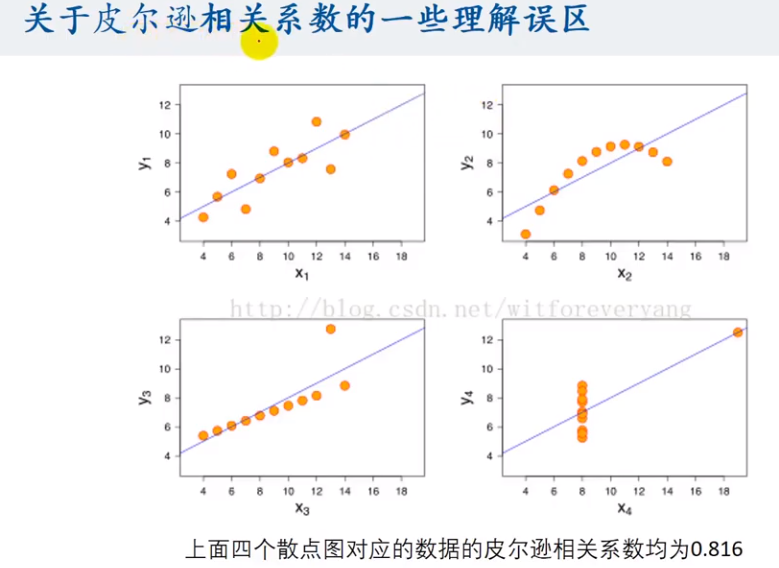
\includegraphics[scale =.5 ]  {figures/interpretation_Pearson_corr.png}}
\end{figure}











\subsubsection{Chebyshev's inequality}
Let $ X $ be a RV with bouned variance:
\begin{equation*}
\mathbb{P}\left( \left\lvert X - E(X) \right\rvert > \varepsilon  \right) \le 
\frac{Var(X)}{\varepsilon^{2}}, \quad \text{ for any } \varepsilon > 0
\end{equation*}
$ X - E(X) $ deviation from the mean.


\subsubsection{Standardize variables}

\begin{equation*}
z = \frac{X - \mu}{\sigma}
\end{equation*}
where $ \mu , \sigma $ are mean and standard deviation. They are {\textbf {constant}}.
Before standardization, 
\begin{align*}
E(X) &= \mu\\
Var(X) &= \sigma^{2}
\end{align*}

After standardization,
\begin{align*}
E(z) &= E \left( \frac{X - \mu}{\sigma} \right)  = \frac{1}{\sigma}E(X - \mu) = \frac{1}{\sigma}
E(\mu - \mu) = 0\\
Var(z)&= Var \left( \frac{X - \mu}{\sigma} \right) = \frac{1}{\sigma^{2}}Var(X - \mu)=
\frac{1}{\sigma^{2}}(Var(X) - 0) = \frac{1}{\sigma^{2}}\sigma^{2} = 1
\end{align*}
After standardization, we have mean 0 and variance 1, rather $ \mu, \sigma $.



\subsection{Higher central moments}

Central moments:
\begin{equation*}
\mu_{r}(\bm{\theta}):=E(X^{r}) = \int_{ - \infty }^{\infty } (x - \mu)^{r}f(x;
\bm{\theta})dx, \quad r = 2,3,...
\end{equation*}
\begin{align*}
\mu_2 &= \mu_2' - (\mu_1')^{2} = \kappa_2 = Variance\\
\end{align*}

\subsubsection{Skewness coefficient}
The skewness coefficient is defined as the standardized third central moments,
\begin{equation*}
\alpha_3(X) = \frac{\mu_3}{(\sqrt {\mu_2})^{3}},\quad \mu_2 = Var = \sigma^{2}
\end{equation*}
If the distribution is {\textbf {symmetric}} around the mean, then,
\begin{equation*}
\alpha_3 = 0.
\end{equation*}
{\textbf {But the reverse does not hold!}} The coefficient of skewness = 0 does not mean
the distribution is symmetric.

If $ \alpha_3 > 0 $, tail on the right.
\begin{figure}[ht]
    \centering
		\scalebox{.7}{\incfig{right-tail}}
    \label{fig:right-tail}
\end{figure}



\subsubsection{Kurtosis}
The Kurtosis coefficient measures peakedness in relation to tails. 
{\textbf {The usefulness of the kurtosis coefficient is reduced if the distribution
is not symmetric.}}

\begin{equation*}
\alpha_4(X) = \frac{\mu_4}{(\mu_2)^{2}}
\end{equation*}
The Kurtosis is the standardized version of the fourth central moment.

We can use the {\textbf {excess kurtosis}} $ (\alpha_4 - 3) $ comparing the peakedness
of a distribution to the Normal distribution.
The Kurtosis of the Normal distribution is 3, i.e., $ \alpha_4 = 3 $.


\begin{itemize}
\item If a distribution is flatter than the Normal distribution, $ \alpha_4 < 3 $.
We call it platykurtic.
\item If a distribution is steeper than the Normal distribution, $ \alpha_4 > 3 $.
We call it leptokurtic.
\end{itemize}
page 119


\subsubsection{Invariance of skewness and kurtosis}

They are invariant to location and scale changes.
For any RV $ X $ whose first four moments exist:
\begin{align*}
\alpha_3(X) &= \alpha_3(a + bX)\\
\alpha_4(X) &= \alpha_4(a + bX)
\end{align*}

\subsubsection{The mode and the median}

The mode for differentiable pdf:
\begin{equation*}
\frac{df(x)}{dx} = 0, \quad s.t., \frac{df^{2}(x)}{dx^{2}}\Bigg|_{x = m_0} < 0
\end{equation*}
Solve for $ x $.



The median, $ x_{\frac{1}{2}} $:
cdf $ F(\cdot ) $
\begin{equation*}
F(x_{\frac{1}{2}}) = \frac{1}{2}, \text{ and $ x_{\frac{1}{2}} $ is unique }
\end{equation*}
solve for $ x $.


\subsubsection{Quantiles}
The $ p $th quantile, denoted by $ x_{p} $:
\begin{equation*}
		F(x_{p}) \ge p, \text{ for } p \in [0,1]
\end{equation*}
Or more formally,
\begin{equation*}
x_{p} := \inf_{x \in \mathbb{R}_{X}}\left\{ x:F_{X}(x) \ge p  \right\} , \text{ for }
p \in (0,1)
\end{equation*}

{\textbf {The value of $ p $ is known as the $ p $th percentile.}}
\begin{itemize}
\item The first quantile (the lower quantile): $ x_{\frac{1}{4}} = F^{-}(0.25) $
\item The third quantile (the upper quantile): $ x_{\frac{3}{4}} = F^{-}(0.75) $
\end{itemize}

The Quantile function
\begin{equation*}
F^{ - }_{X}(\cdot ): (0,1)\rightarrow \mathbb{R}_{X}
\end{equation*}
It is not the same as the inverse function $ F^{ - 1}_{X}(\cdot ) $.
The inverse function exists only if the cdf is one-to-one, continuous and strictly
increasing.



\subsubsection{The inverse probability integral transformation}
For any continuous RV $ X $ with cdf such that $ u = F_{X}(x) $ is invertible, 
i.e., $ x = F^{ - 1}(u) $, we can make the transformation.

Example:

For RV $ u = F(X) $ follows uniform distribution
\begin{equation*}
u = F(X) \sim U(0,1)
\end{equation*}
we want to transform it into an exponentially distributed RV $ X $ with 
\begin{equation*}
F(x) = 1 - e^{ - \theta x}, \quad x > 0
\end{equation*}
we can let $ u = 1 - e^{ - \theta x} $, then
\begin{align*}
e^{ - \theta x} &= 1 - u\\
x &= F_{X}^{ - 1}(u) =  \frac{1}{\theta}\ln (1 - u), \quad u \in (0,1)
\end{align*}

This result can be used to simulate exponentially distributed RVs using uniformly
distributed RVs.




\subsection{Inequalities}

\subsubsection{General Chebyshev's inequality}
Let $ X(.): S \rightarrow \mathbb{R}_{X}:=(0, \infty ) $ be a positive RV. Let
$ g(.):(0,\infty ) \rightarrow (0,\infty ) $ be a positive and increasing function.
Then for each $ \varepsilon > 0 $:
\begin{equation*}
\mathbb{P}(g(X) \ge  \varepsilon)	\le \frac{E(g(X))}{g(\varepsilon)}
\end{equation*}


\subsubsection{Markov's inequality}
Let $ X $ be a RV such that $ E(\left\lvert X \right\rvert^{p} ) < \infty $, for
$ p > 0 $:
\begin{equation*}
\mathbb{P}(\left\lvert X \right\rvert  \ge  \varepsilon) \le  
\frac{E(\left\lvert X \right\rvert ^{p})}{\varepsilon^{ p}}
\end{equation*}
When $ X $ equals to $ X - E(X) $ and $ p = 2 $, we receive
\begin{equation*}
\mathbb{P}(\left\lvert X - E(X) \right\rvert \ge  \varepsilon ) \le  
\frac{Var(X)}{\varepsilon^{2}}, \quad \text{ for any  } \varepsilon > 0
\end{equation*}


\subsubsection{Jensen's inequality}

Let $ \varphi(\cdot ): \mathbb{R} \rightarrow \mathbb{R}  $ be a convex function
\begin{equation*}
\lambda \varphi(x) + (1 - \lambda)\varphi(y) \ge  \varphi(\lambda x + (1 - \lambda y))
, \quad \lambda \in (0,1), x, y \in \mathbb{R}
\end{equation*}

\begin{figure}[ht]
    \centering
		\scalebox{.5}{\incfig{convex}}
    \label{fig:convex}
\end{figure}



\section{Joint Distribution}
Two continuous RV, $ X, Y $,
\begin{align*}
		\mathbb{P}(s:X(s) \le x) &= P_{X}(( - \infty , x]) = F_{X}(x), \quad x \in \mathbb{R}\\
		\mathbb{P}(s:Y(s) \le y) &= P_{Y}(( - \infty , y]),= F_{Y}(y), \quad  y \in \mathbb{R}\\
\end{align*}

The {\textbf {joint cdf}} is defined by:
\begin{align*}
		F_{XY}(.,.)&: \mathbb{R}^{2} \rightarrow [0,1]\\
		F_{XY}(x,y) = \mathbb{P}\left\{ s:X(s) \le x, Y(s) \le y \right\} &= P_{XY}(
		( - \infty ,x] \times ( - \infty , y]), \quad (x,y) \in \mathbb{R}^{2}
\end{align*}

\begin{equation*}
F(x,y) = \int_{ - \infty }^{x}\int_{ - \infty }^{y} f(u,v)du dv 
\end{equation*}
where $ f(x,y) > 0 $ is known as the {\textbf {joint density function}}.

If $ F(\cdot ) $ is differentiable, we can derive the join density by
\begin{align*}
f(x,y) = \frac{\partial^{2}F(x,y)  }{\partial x \partial y }
\end{align*}
\noindent\fbox{%
\parbox{\textwidth}{%
Example:\\
Given the joint cdf of the bivariate Exponential distribution:
\begin{equation*}
F(x,y) = 1 - e^{ - x} - e^{ - y} + e^{ - x - y},
\end{equation*}
The joint density can be derived by
\begin{align*}
\frac{\partial F(x,y) }{\partial x }&= e^{ - x} - e^{ - x - y}\\
\frac{\partial^{2}F(x,y)  }{\partial x \partial y }&= e^{ - x - y}
\end{align*}
where $ x, y \ge 0 $
}%
}\\

In the univariate case, {\textbf {the joint density takes values greater than one,
i.e., }}
\begin{equation*}
		f(.,.) : \mathbb{R} \times \mathbb{R} \rightarrow [0, \infty )
\end{equation*}

\subsection{Properties of the join density}
\begin{itemize}
\item $ f(x,y) \ge 0, \forall (x,y) \in \mathbb{R}_{X} \times \mathbb{R}_{Y}$ 
\item $ \int_{ - \infty }^{\infty } \int_{ - \infty }^{\infty }f(x,y)dx dy  = 1 $
\item $ F_{XY}(a,b) = \int_{ - \infty }^{a}\int_{ - \infty }^{b}f(x,y)dydx   $
\item In the discrete case:
\item $ \sum\limits_{i = 1} ^\infty \sum\limits_{j = 1} ^\infty f(x_{i},y_{j}) = 1 $
\item $ F(x_{k},y_{m}) = \sum\limits_{i = 1} ^k \sum\limits_{j = 1} ^m f(x_{i},y_{j})		 $
\end{itemize}




\bibliographystyle{plainnat}
\bibliography{my_bib}

\end{document}

